\documentclass[a4paper]{article}
\usepackage{tikz}
\usetikzlibrary{arrows,backgrounds,positioning,calc,fit,shapes.geometric,decorations.pathreplacing,decorations.markings}
\usepackage{geometry}
\usepackage{siunitx}
\usepackage{graphicx}
\usepackage{natbib}
\usepackage{amsmath}
\usepackage{amssymb}
\usepackage{amsthm}
\usepackage{paralist}
\usepackage{epstopdf}
\usepackage{tabularx}
\usepackage{longtable}
\usepackage{multirow}
\usepackage{multicol}
\usepackage[hidelinks]{hyperref}
\usepackage{fancyvrb}
\usepackage{algorithm}
\usepackage{algorithmic}
\usepackage{float}
\usepackage{paralist}
%\usepackage[svgname]{xcolor}
\usepackage{enumerate}
\usepackage{array}
\usepackage{times}
\usepackage{url}
\usepackage{fancyhdr}
\usepackage{comment}
\usepackage{environ}
\usepackage{times}
\usepackage{textcomp}
\usepackage{caption}
\usepackage{bbm}


\urlstyle{rm}

\setlength\parindent{0pt} % Removes all indentation from paragraphs
\theoremstyle{definition}
\newtheorem{definition}{Definition}[]
\newtheorem{conjecture}{Conjecture}[]
\newtheorem{example}{Example}[]
\newtheorem{theorem}{Theorem}[]
\newtheorem{lemma}{Lemma}
\newtheorem{proposition}{Proposition}
\newtheorem{corollary}{Corollary}

\floatname{algorithm}{Procedure}
\renewcommand{\algorithmicrequire}{\textbf{Input:}}
\renewcommand{\algorithmicensure}{\textbf{Output:}}
\newcommand{\abs}[1]{\lvert#1\rvert}
\newcommand{\norm}[1]{\lVert#1\rVert}
\newcommand{\RR}{\mathbb{R}}
\newcommand{\CC}{\mathbb{C}}
\newcommand{\Nat}{\mathbb{N}}
\newcommand{\br}[1]{\{#1\}}
\DeclareMathOperator*{\argmin}{arg\,min}
\DeclareMathOperator*{\argmax}{arg\,max}
\renewcommand{\qedsymbol}{$\blacksquare$}

\definecolor{dkgreen}{rgb}{0,0.6,0}
\definecolor{gray}{rgb}{0.5,0.5,0.5}
\definecolor{mauve}{rgb}{0.58,0,0.82}

\definecolor{C0}{HTML}{1F77B4}
\definecolor{C1}{HTML}{FF7F0E}
\definecolor{C2}{HTML}{2ca02c}
\definecolor{C3}{HTML}{d62728}
\definecolor{C4}{HTML}{9467bd}
\definecolor{C5}{HTML}{8c564b}
\definecolor{C6}{HTML}{e377c2}
\definecolor{C7}{HTML}{7F7F7F}
\definecolor{C8}{HTML}{bcbd22}
\definecolor{C9}{HTML}{17BECF}

\newcommand{\Var}{\mathrm{Var}}
\newcommand{\Cov}{\mathrm{Cov}}
\newcommand{\sgn}{\mathrm{sgn}}

\newcommand{\vc}[1]{\boldsymbol{#1}}
\newcommand{\xv}{\vc{x}}
\newcommand{\Sigmav}{\vc{\Sigma}}
\newcommand{\alphav}{\vc{\alpha}}
\newcommand{\muv}{\vc{\mu}}

\newcommand{\red}[1]{\textcolor{red}{#1}}

\def\x{\mathbf x}
\def\y{\mathbf y}
\def\w{\mathbf w}
\def\v{\mathbf v}
\def\E{\mathbb E}
\def\R{\mathbb R}
\def\V{\mathbb V}
\def\ind{\mathbbm 1}

% TO SHOW SOLUTIONS, include following (else comment out):
\newenvironment{soln}{
	\leavevmode\color{blue}\ignorespaces
}{}


\hypersetup{
	%    colorlinks,
	linkcolor={red!50!black},
	citecolor={blue!50!black},
	urlcolor={blue!80!black}
}

\geometry{
	top=1in,            % <-- you want to adjust this
	inner=1in,
	outer=1in,
	bottom=1in,
	headheight=3em,       % <-- and this
	headsep=2em,          % <-- and this
	footskip=3em,
}


\pagestyle{fancyplain}
\lhead{\fancyplain{}{Homework 7}}
\rhead{\fancyplain{}{CS 760 Machine Learning}}
\cfoot{\thepage}

\title{\textsc{CS 760 Final Project\\Applications of Machine Learning for Algorithmic Redistricting}} % Title

%%% NOTE:  Replace 'NAME HERE' etc., and delete any "\red{}" wrappers (so it won't show up as red)

\author{
	\red{Daniel Szabo} \\
	\red{9074762189}\\
} 

\date{}

\begin{document}
	
	\maketitle 
	
	\section{Introduction}
	In this paper I'll analyze some methods for quantifying gerrymandering using machine learning. Theoretically I will assume we are given a truly uniform random representative sample of all possible districting plans of some geographic entity, and then discuss what can be done to extract information relevant to the study of gerrymandering from this sample. This includes using unsupervised learning to see the structure and significance of certain gerrymandering metrics from the political science literature, as well as using supervised learning to identify gerrymandering with CNNs.
	
	\section{Background and Data}
	
	Gerrymandering is the partisan process of drawing election maps in particular ways to gain a political advantage, and results in the disenfranchisement voters. It is a central issue in political science that has no clear solution, and remains a contentious issue in courts all over the United States. One of the key difficulties is quantifying gerrymandering in a way that can hold up in court. The most popular solution to this is currently to draw a \emph{representative} sample of all possible elections maps (districting plans) and use those to classify a given plan as gerrymandered or not. Usually this is done using one of the many metrics available in the political science literature, and conducting a statistical test for the significance of whether the given plan comes from the sampled distribution.
	
	Algorithmic redistricting refers to the methods for sampling districting plans. This has mostly been done with Markov Chain Monte Carlo algorithms \cite{ReCom}, but also using topological data science \cite{TDS}, as well as methods from statistical mechanics \cite{StatPhys}. One of the issues with all of these methods is that they have no theoretical justification to being a representative sample of the space of all possible legislative maps, which is huge. My work with Jin-Yi Cai, Ashwin Maran, Kenneth Mayer and Song Gao among others has resulted in a new algorithm that can truly uniformly sample from this space by counting exactly the total number of possible partitions, and using that to sample in subexponential time (in the number of precincts).
	
	More formally, we are given a planar adjacency graph $ G $ where vertices are precincts (the building blocks of districts) and can sample a non-self-intersecting path $ p $ on the edges of $ G $. Because each edge corresponds to a boundary between two districts, $ p $ is also a path on the edges of $ H $, the dual of $ G $, where precincts are faces-- this corresponds to an actual map we are used to seeing. 
	
	A significant political caveat to this entire field is that partisan gerrymandering is not currently illegal. In 2019 the supreme court ruled in Rucho v. Common Cause that only the supreme court can regulate claims for gerrymandering, and other cases showed that they can only really decide based on racial disenfranchisement. In other words, even if we were to show that some map is drawn in a completely partisan way, if it does not intentionally disenfranchise a target population, it is not illegal. Nonetheless the mathematics of this area remains interesting, as the distinction remains a very gray area.
	
	\subsection{Data}\label{data}
	
	Unfortunately the practical case for sampling is quite different from the theory. The data comes from legislative districts 26 and 27 near Sheboygan, WI from the 2012 election, and only looks at approximately 200 precincts. The algorithm to sample districting plans currently is only implemented for partitioning into 2 districts. Thus I am trying to measure gerrymandering using a relatively small republican majority area that can only be split into two districts, a case for which many of the most popular metrics may not even have any significance. The algorithm to sample districting plans produced 3446 sample plans out of the enormous space of 6080174112134899589734 possible plans.
	
	Another issue is with the nature of the underlying geographic data. Precincts are drawn by humans and modified slightly over time for a plethora of reasons, and often have inconsistencies. Because of this the requirement for the population of each district to be similar had to be waived, as the real districting plan did not adhere to those requirements either. This means we are sampling from a much larger space that is not really representative of any districting plans, but the methods here can still be applied to better data.
	
	For supervised learning, I used 33 images from Dr. Mayer's 2018 Expert Report \cite{KenExpert} on specific Assembly districts in Wisconsin to train the CNN. There he describes how these plans are gerrymandered, and gives alternate districting plans as well. The images came from a word document, and had some errors or inconsistencies that I did not know how to heal.
	
	\subsection{Metrics}
% [efficiency, mean_meadian, mean_thirdian, partisan bias, partisan Gini score, polsby-popper compactness, population1, population2]	
	The metrics I used were mostly those available from the Metric Geometry and Gerrymandering Group's (MGGG) GerryChain algorithm \cite{ReCom}. They include the efficiency gap, population, vote percentage, partisan Gini score, and Polsby-Popper compactness.
	\begin{itemize}
		\item[Efficiency Gap:] The efficiency gap is a measure of each party's wasted votes. It is	calculated as the difference in the two parties’ total wasted votes, divided by the total number of votes cast.
		\item[Vote Percentage:] The vote percentage is only applicable for two districts, and simply measures the difference between the largest percentage of votes won in a district and the average percentage of the two districts.
		\item[Partisan Gini Score:] The partisan Gini score is defined as the area between the seats-votes
		curve and its reflection about $ f(x)=x $. The seats-votes curve plots the percentage of seats a party controls as a function of its share of the overall vote summed across all districts.
		\item[Population:] Due to the difficulties mentioned in Section \ref{data}, it is also relevant to collect the population of each district.
		\item[Polsby-Popper compactness:] The only compactness measure I collect is the Polsby-Popper score $ PP $, which is the following ratio of the area $ A $ of a district and its perimeter $ P $:
		\[ PP = \frac{4\pi A}{P^2}. \]
	\end{itemize}
	
	\section{Unsupervised Learning}
	The space of metrics evaluated from the sampled redistricting plans is inherently unlabeled. Using this data, we want to say something about the single real districting plan. Previous methods simply look at where the true plan lies in this distribution, however after visualizing a 2-dimensional embedding generated by PCA, it seemed the data was naturally clustered, so I tried using $ k $-means to get a sample space that better represents the behavior of these metrics within a cluster.
	
	\subsection{Hypothesis}
	The statistical behavior within a $ k $-means cluster is a good predictor of whether a districting plan is gerrymandered.
	
	\subsection{Methods}
	First, to choose the hyperparameter $ k $, I used principal component analysis to visualize the metrics. The reasoning is that the different metrics measure similar aspects of the data, so it likely can be well represented by some lower dimensional space. To implement this, I used sklearn's PCA algorithm \cite{scikit-learn}.
	
	After choosing $ k $, we need to implement $ k $-means, which I also did using sklearn. The computational benefits of the lower dimensional embeddings are not necessary as we only collected $ 8 $ metrics, so we can use the original data after normalization.
	
	Once we have a clustering, we can look at the behavior of our sample within its cluster. Although this can be done using multivariate analysis, a simpler approach is to see where it lies in the distribution of signed distances from the cluster center. The sign of the euclidean distance to the center can be determined by which side it is of any hyperplane crossing the center, as it's only needed for the distribution of distances to be approximately normal (symmetric).
	
	\subsection{Results}
	The singular values suggested that the districting plans could be well represented in two dimensions. These dimensions may correspond to partisan metrics versus compactness metrics, as those are significantly different while partisan metrics tend to be correlated. The singular values were approximately
	\[ [\num{2.0107e+06}, \num{9.0811e+05}, \num{6.5658e+00}, \num{8.6638e-01}, \num{6.8599e-01}, \num{3.5867e-01}, \num{1.2918e-01} ]. \]
	The 2-dimensional visualization in the largest two eigenbases is shown in Figure \ref{fig1}. This suggests a choice of $ k=5 $ would be appropriate.
	
	\begin{figure}[h]
		\centering
		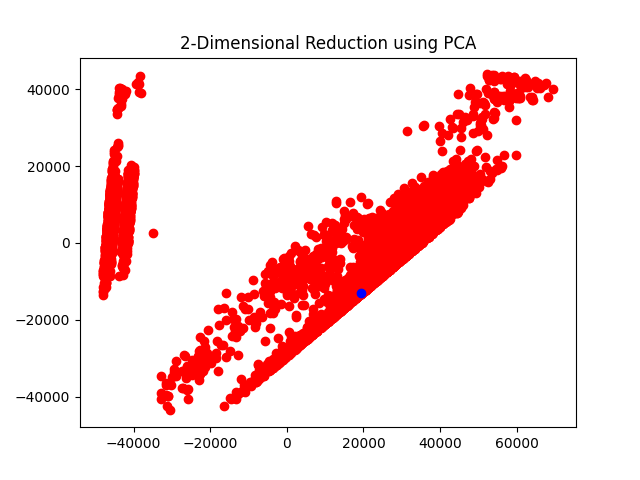
\includegraphics[scale=.4]{2Dvisual.png}
		\caption{The lower dimensional representation of the randomly sampled metric data. The red dots represent sampled plans, and the blue dot the existing districting plan.}\label{fig1}
	\end{figure}

	The distribution of the cluster along with the current districting plan can be seen in Figure \ref{fig2}.
	
	\begin{figure}[h]
		\centering
		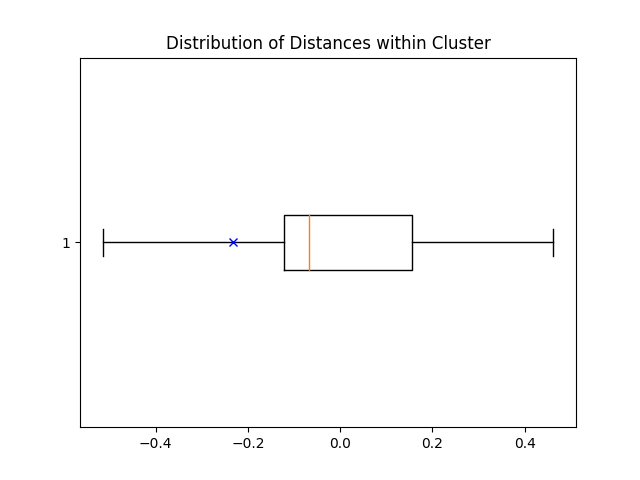
\includegraphics[scale=.4]{boxplot.png}
		\caption{The location of the existing districting plan (labeled by a blue x) in the distribution of signed Euclidean distances.}\label{fig2}
	\end{figure}

	\subsection{Analysis}
	We do not have a realistic enough example to accept or refute our hypothesis.
	
	The reason the data is clustered as seen in Figure \ref{fig1} is not inherent to the problem, but to the particular samples. They were generated by going over all possible ``opposite" starting and ending points for the district border, and looking at the statistics of the ordered samples it is clear that the clusters are due to the location of these starting and ending points. Nonetheless it is known that larger samples the space of districting plans is in some way clustered, as it is one of the shortcomings of algorithms that can only optimize locally (exploit rather than explore).
	
	The actual example failed to correctly classify the real districting plan that was gerrymandered, however the methodology still has potential in larger instances.
	
	\section{Supervised Learning}
	For my supervised learning approach, I trained a convolutional neural network on images of districting plans.
	
	\subsection{Hypothesis}
	A CNN trained on labeled images of districting plans is a good predictor of gerrymandering.
	
	
	\subsection{Methods}
	Before training, we need to transform the images to a regular size. I chose a smaller size of 3$ \times $100$ \times $100, as the most important feature we had to preserve in these images were the boundaries. I would have then liked to somehow increase the contrast of these boundaries so the network treats them with more weight, however I could not find a way to do that with the data already having some faults. The transformed data can be seen in Figure \ref{fig3}.
	
	
	\begin{figure}[h]
		\centering
		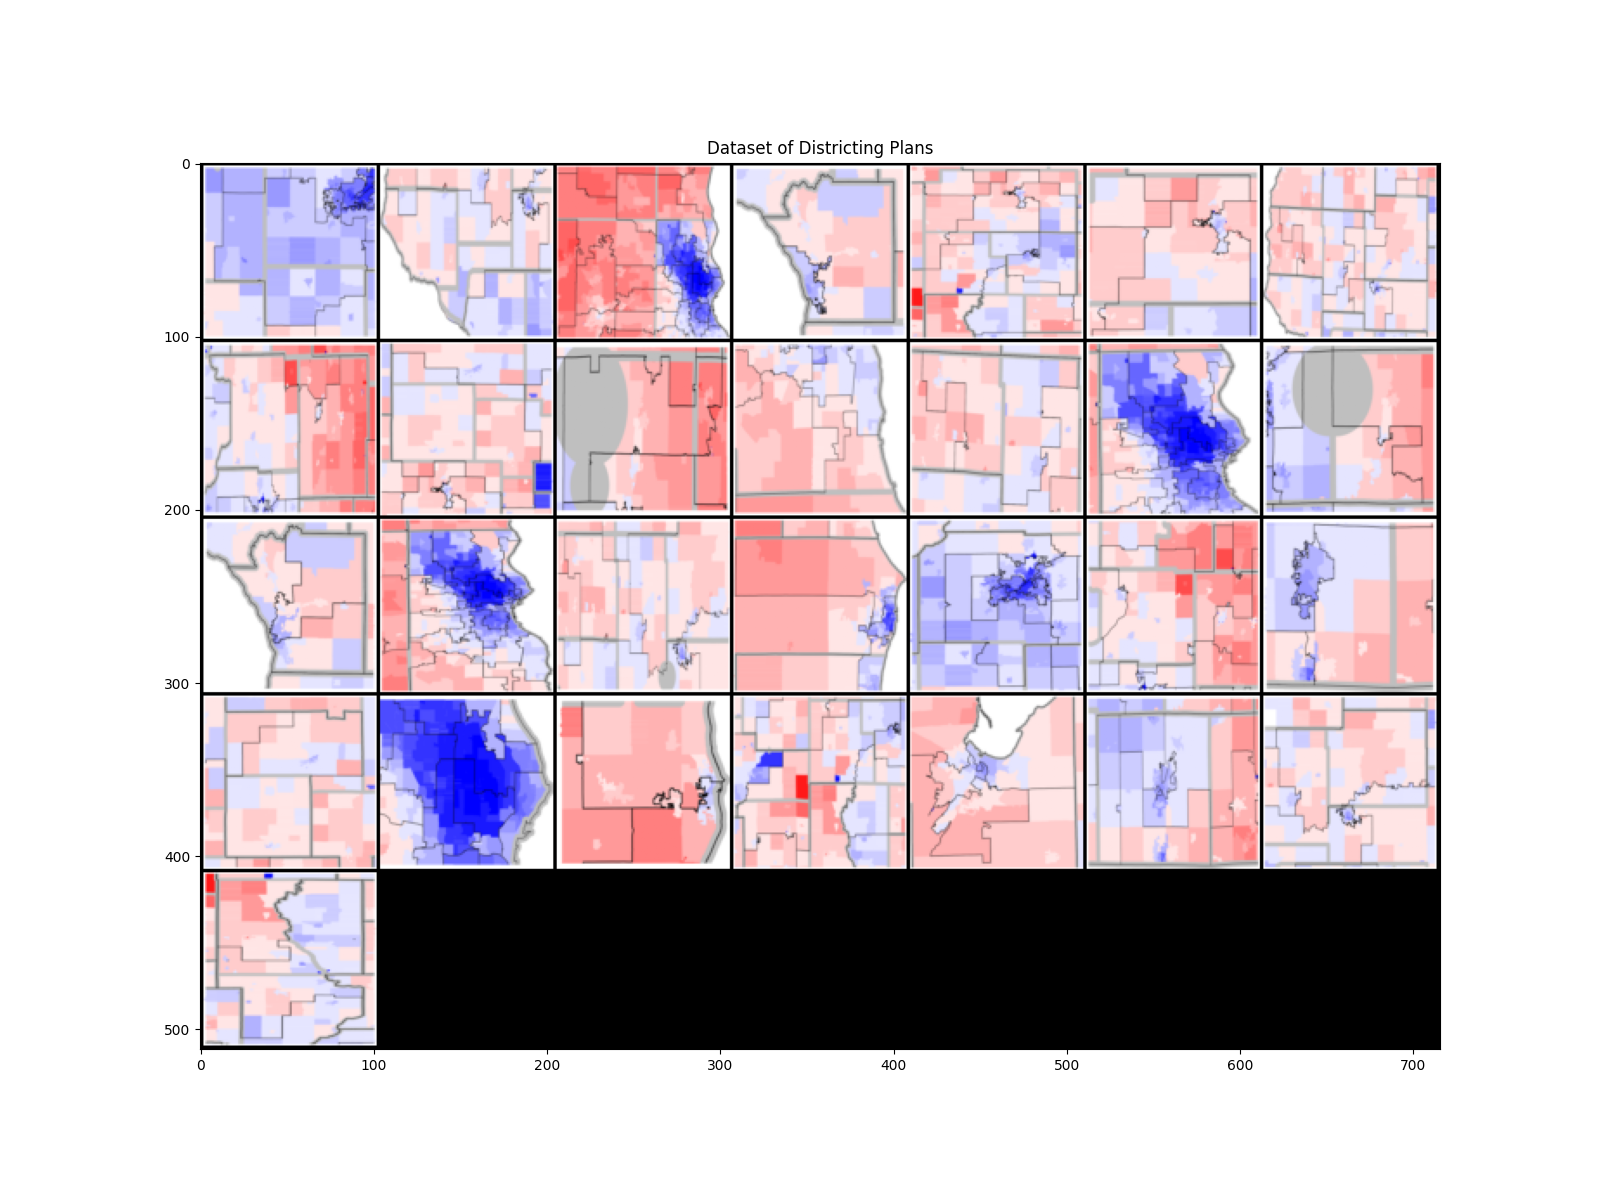
\includegraphics[scale=.3]{plans.png}
		\caption{Images of current gerrymandered districts and alternative fair districting plans in an arbitrary ordering.}\label{fig3}
	\end{figure}

	Then after sampling a training and validation set, the CNN has the following structure:\\
	We first have two similar convolution blocks that increase the dimension to $ 64\times 100\times 100 $ using small ($ 3\times 3 $) kernels in an effort to highlight the sharp local features, the boundaries. ReLU activation is used between layers. Then I tried using a convolution layer that preserves the dimension however has a large kernel to account for larger scale relationships. Between convolution blocks I used max pooling layers. Finally, I reduce the dimension to the output dimension of 2 with 3 fully connected linear layers.
	
	Training was done using SGD and cross-entropy loss over 50 epochs with a learning rate of $ 0.01 $. The batch size had to be low due to the small number of samples (33), only being 4. Cross-validation showed that changing these hyperparameters did not significantly improve results.
	
	\subsection{Results}
	Due to the small number of samples, the validation set could not be too large and still be independent from the training set, so validation accuracy was not the best metric. Instead I used the loss function of the CNN, which is plotted in Figure \ref{fig4}. Despite the relatively small learning rate and high number of epochs, the loss showed no sign of converging to anything with good accuracy.

	\begin{figure}[h]
		\centering
		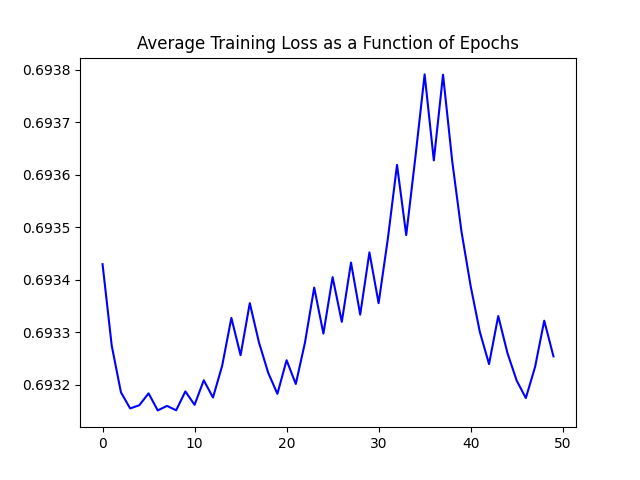
\includegraphics[scale=.4]{loss.png}
		\caption{The average training loss of the CNN per epoch.}\label{fig4}
	\end{figure}

	\subsection{Analysis}
	Although there are other confounding factors, the CNN could not effectively detect gerrymandering on this dataset.
	
	Not only was the dataset too small, but the CNN had no way of identifying which feature of these maps was important. This could have been solved by pairing the data points in some way (as in, say, a paired $ t $-test in statistics because the original data was paired), or using a more sophisticated model that knows to focus on the boundary lines rather than the underlying voter distribution.
	
	There is also a deeper issue of what is defined as gerrymandering. It is not always the case that straighter boundaries that seem uncorrelated to the underlying voter distribution are not gerrymandered, despite this being the usual adhoc definition. Geographic data can inherently have strange nonlinear boundaries, and because of this gerrymandering is better measured by the outcomes of elections being far from the actual voters' percentages.
	
	Nonetheless neural networks can learn surprising things, and this experiment alone is not enough to refute the potential of artificial intelligence in detecting gerrymandering. With larger quantities of more thorough and carefully processed data, some deeper networks could be able to learn the features necessary to identify gerrymandering.

	\bibliographystyle{plain}
	\bibliography{refs.bib}	
	
\end{document}
